\documentclass[tikz,border=5pt]{standalone}

\begin{document}
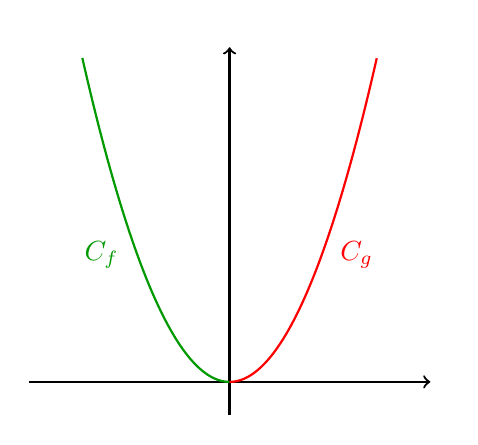
\begin{tikzpicture}[x=0.85cm,y=0.85cm, thick]

  % Axes
  \draw[->] (-3,0) -- (3,0) node[right] {};
  \draw[->] (0,-0.5) -- (0,5) node[above] {};

  % Negative half of y = x^2 (green)
  \draw[green!60!black, thick, variable=\t, domain=-2.2:0, samples=120]
    plot ({\t}, {\t*\t});

  % Positive half of y = x^2 (red)
  \draw[red, thick, variable=\t, domain=0:2.2, samples=120]
    plot ({\t}, {\t*\t});

  % Graph labels
  \node[green!60!black, below left] at (-1.5,2.25) {$C_f$};
  \node[red, below right] at (1.5,2.25) {$C_g$};

\end{tikzpicture}
\end{document}
